\begin{frame}{Visão geral do software}

\end{frame} 

\begin{frame}{Representação visual}

\end{frame}

\begin{frame}{Árvore de expressões}

\end{frame}

\begin{frame}{Representação intermediária}

\end{frame}

% \begin{frame}{Fluxograma de uso simplificado}
%     \begin{figure}
%         \centering
%         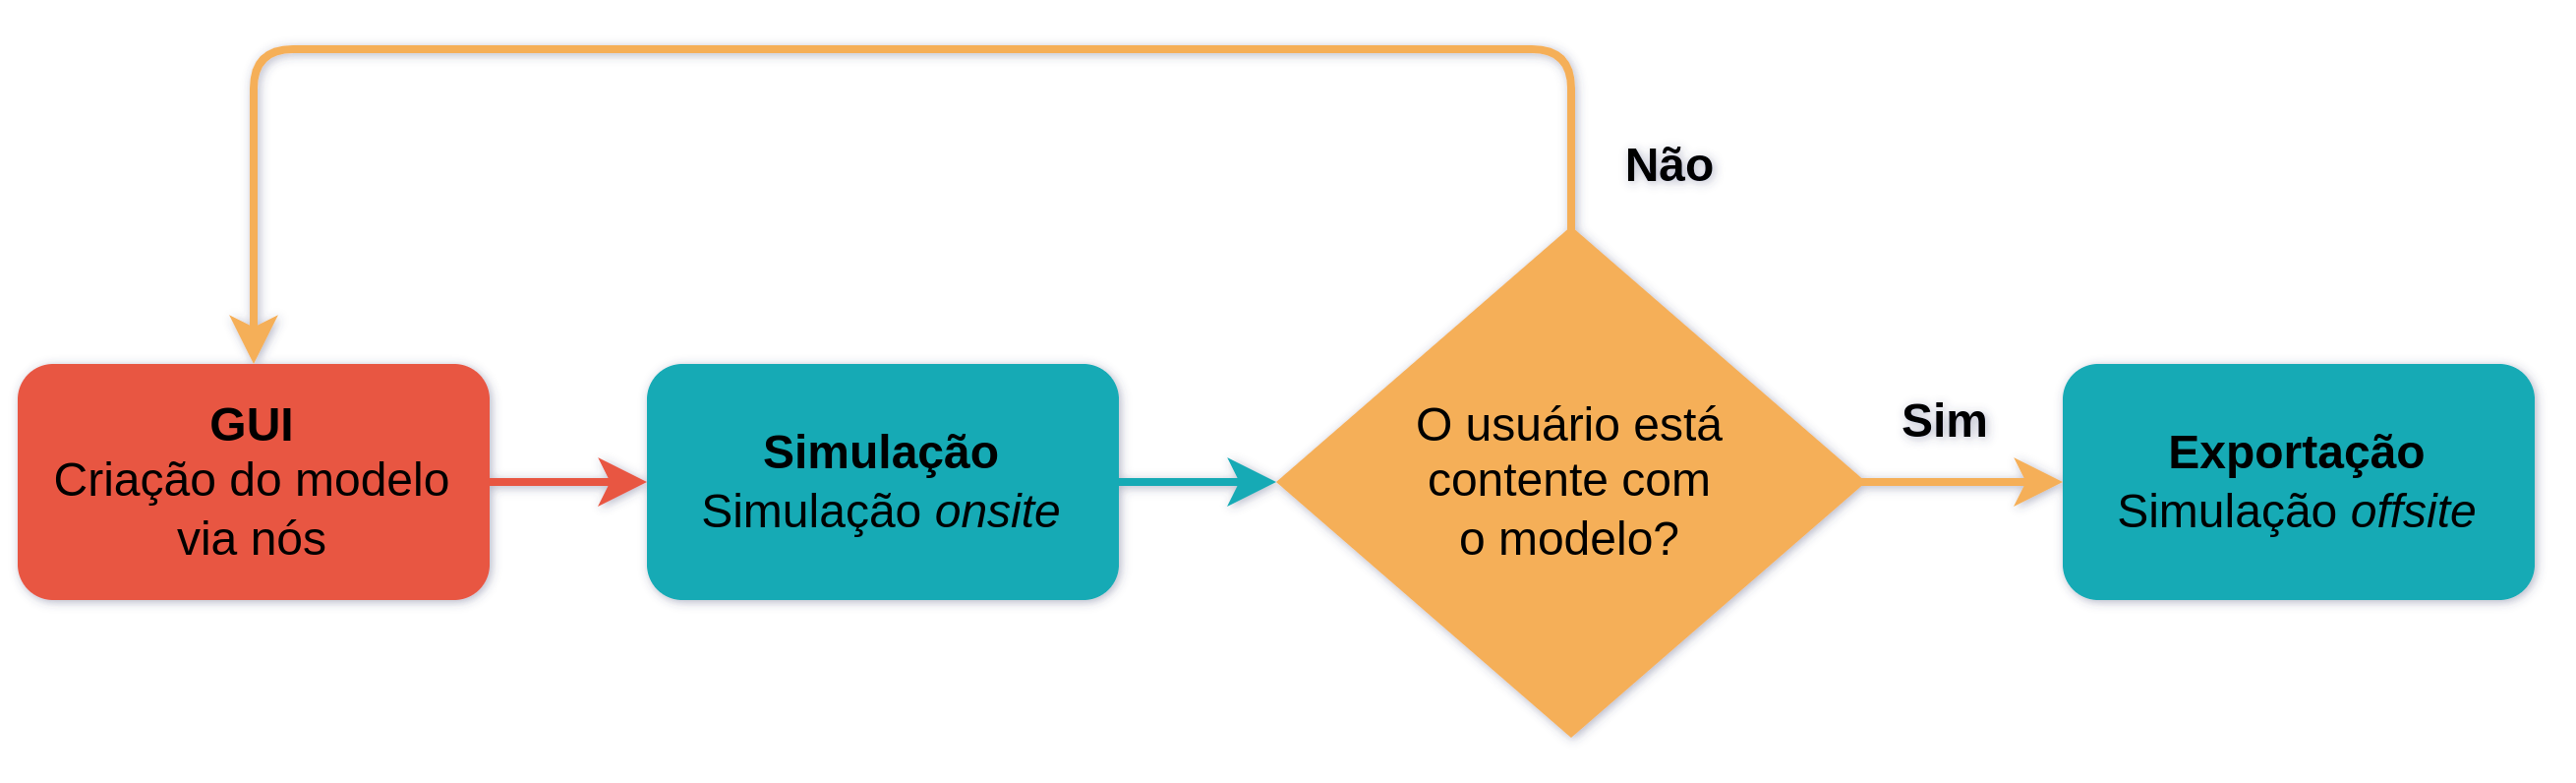
\includegraphics[width=\textwidth, height=\textheight, keepaspectratio=true]{beamerthemesrc/images/ode-designer-fluxograma.png}
%         \caption{Fluxograma da experiência do usuário.}
%     \end{figure}
% \end{frame}

% \begin{frame}{Funcionalidades do Software}
%     O software deve entregar as seguintes funcionalidades:
%     \begin{itemize}
%         \item Criação de modelos pela interface gráfica;
%         \item Simulação do modelo e exibição dos resultados na interface;
%         \item Exportação de PDF/Imagens com os resultados das simulações;
%         \item Exportação de código equivalente ao modelo implementado;
%     \end{itemize}
% \end{frame}

% \subsection{Interface Gráfica}

% \begin{sidepic}{beamerthemesrc/images/ode-designer-gui-exemplo}{Representação do Modelo}
%     \begin{itemize}
%         \item O software necessita de uma interface simples de ser usada;
%             \begin{itemize}
%                 \item Mas também deve naturalmente relembrar uma EDO;
%             \end{itemize}
%         \item Após diversas iterações, chegamos numa interface baseada em programação visual;
%             \begin{itemize}
%                 \item Estas interfaces existem desde 1963, mas tiveram uma renascença com o avanço dos computadores e a necessidade de softwares de edição de imagem/áudio/vídeo;
%             \end{itemize}
%     \end{itemize}
% \end{sidepic}

% \begin{frame}{Fluxo de passagem de informações na interface}
%     \begin{figure}
%         \centering
%         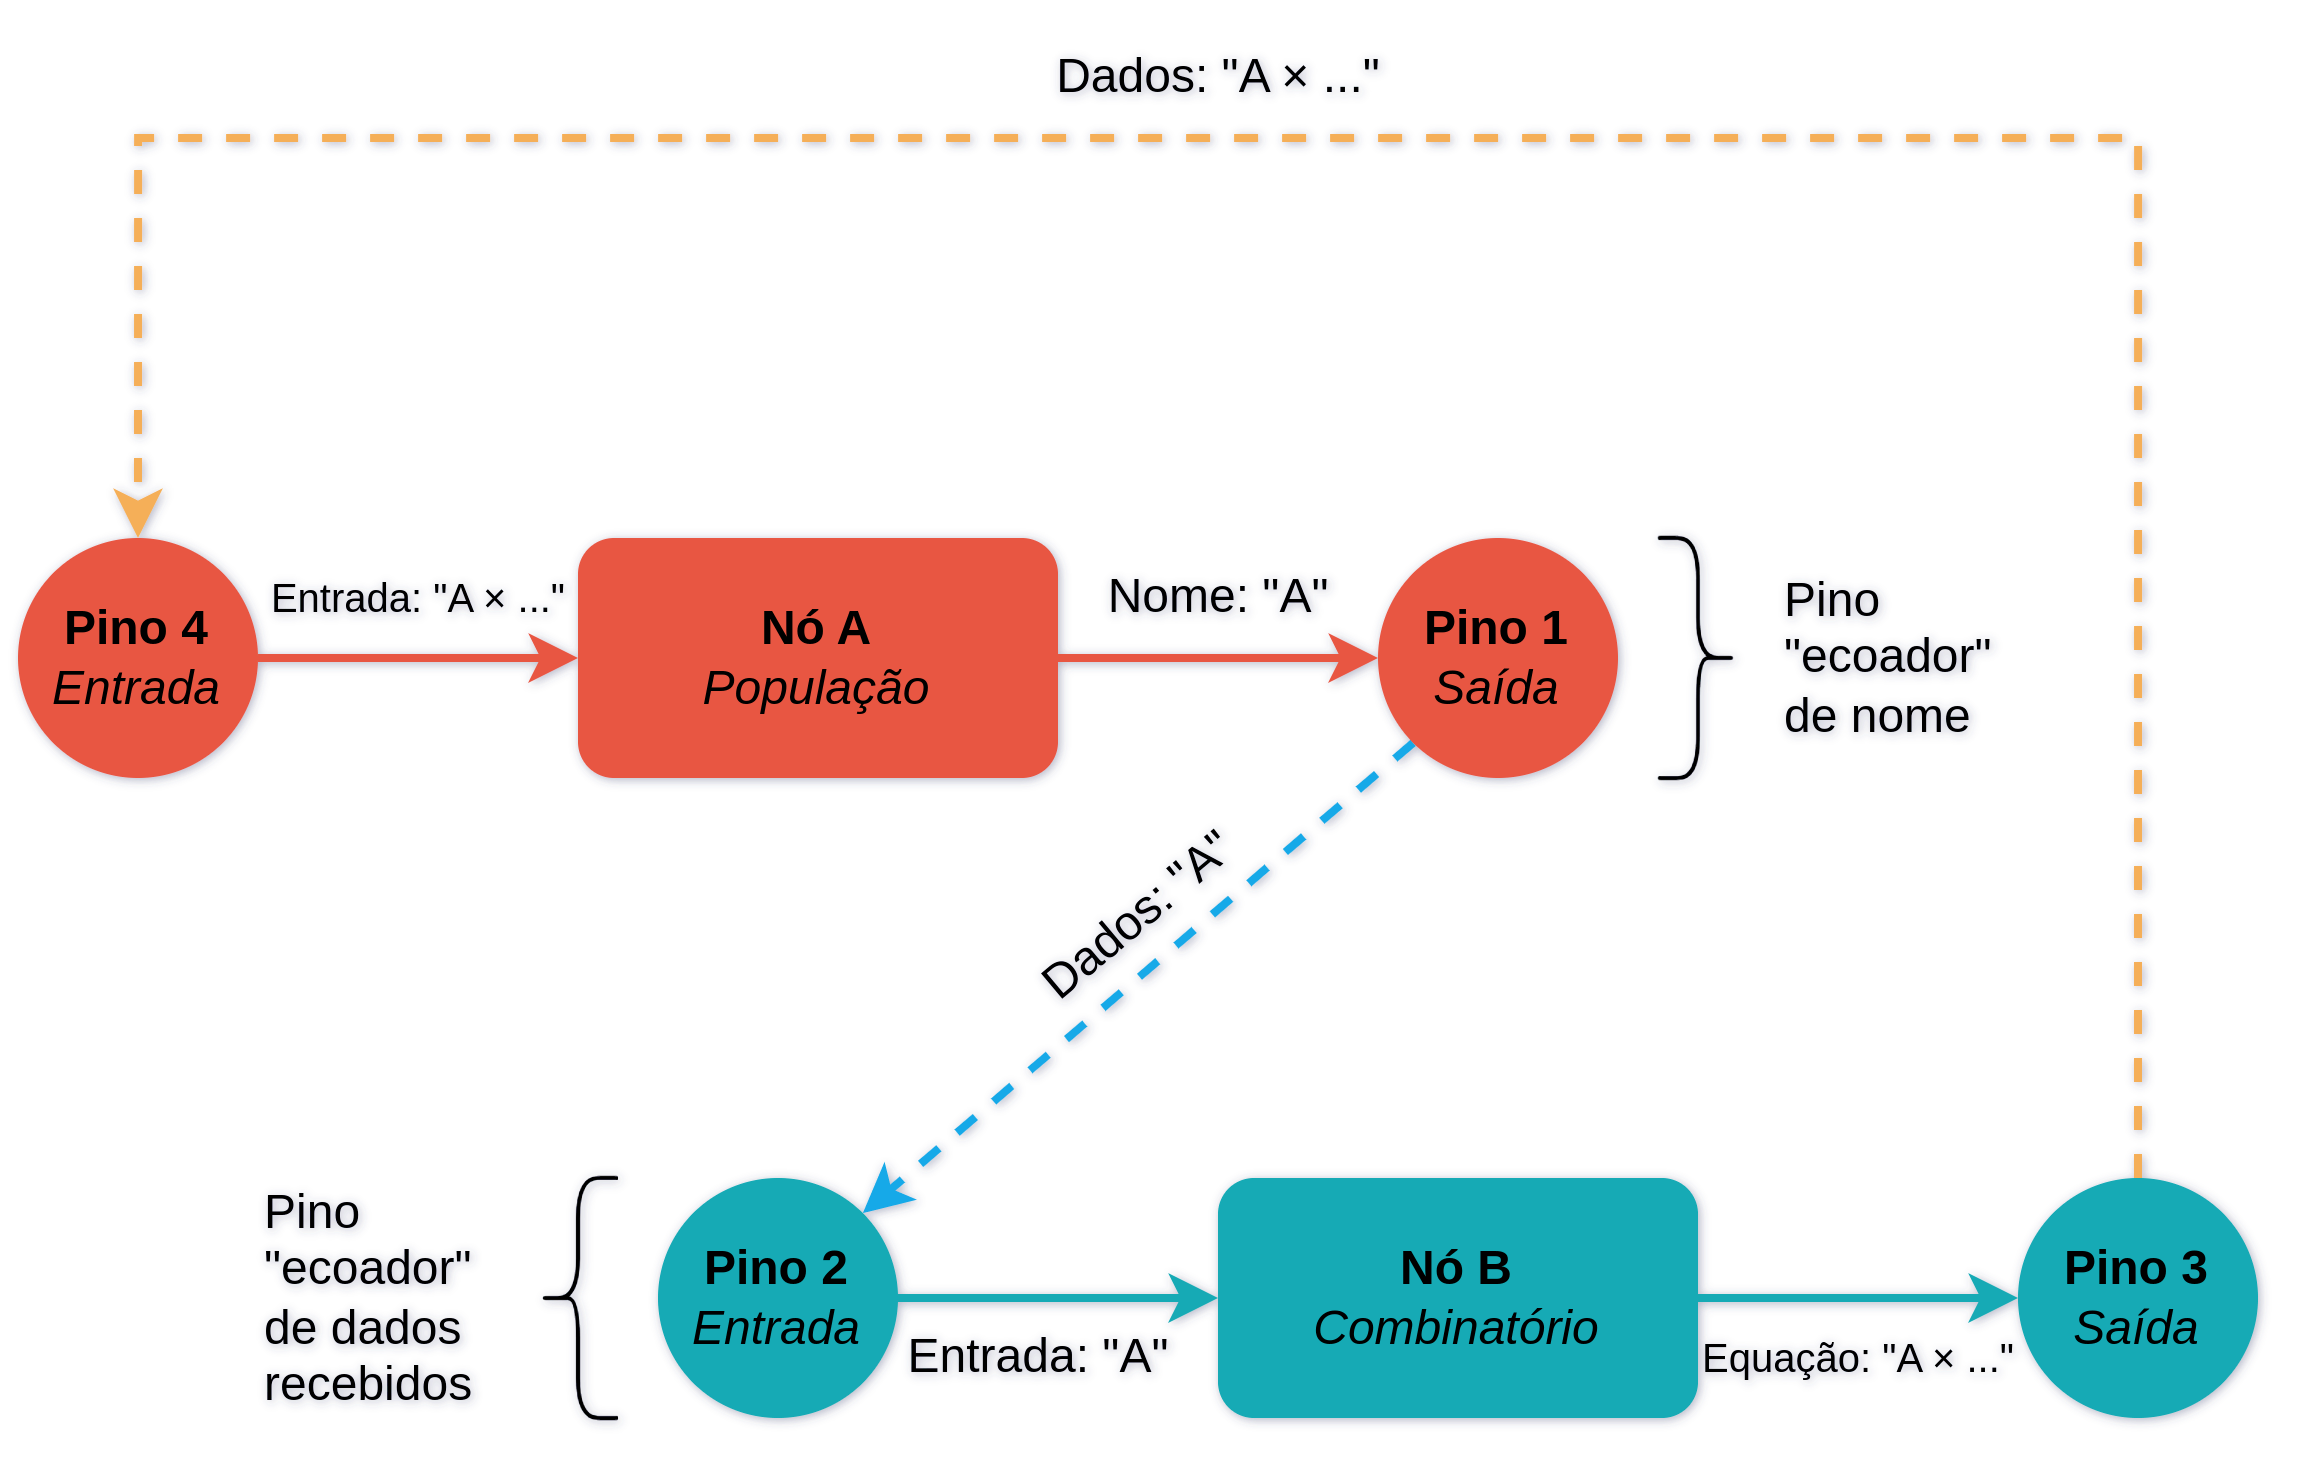
\includegraphics[width=\textwidth, height=\textheight, keepaspectratio=true]{beamerthemesrc/images/fluxo-dados-gui.png}
%         \caption{Relações entre nós e pinos.}
%     \end{figure}
% \end{frame}

% \subsection{Representação Intermediária}

% \begin{chapter}[beamerthemesrc/assets/background_negative]{}{Representação Intermediária}
% \end{chapter}

% \begin{frame}{Representação Intermediária}
%     \begin{itemize}
%         \item Com o objetivo de realizar tantas transformações, torna-se necessário a utilização de uma Representação Intermediária (RI);

%         \item Inspirados nas arquiteturas de compiladores modernos (GCC, baseados em LLVM), separamos a estrutura em back-end e front-end;

%         \item Essa abordagem garante o desacoplamento entre estrutura e produtos finais;
%     \end{itemize}

%     \begin{figure}
%         \centering
%         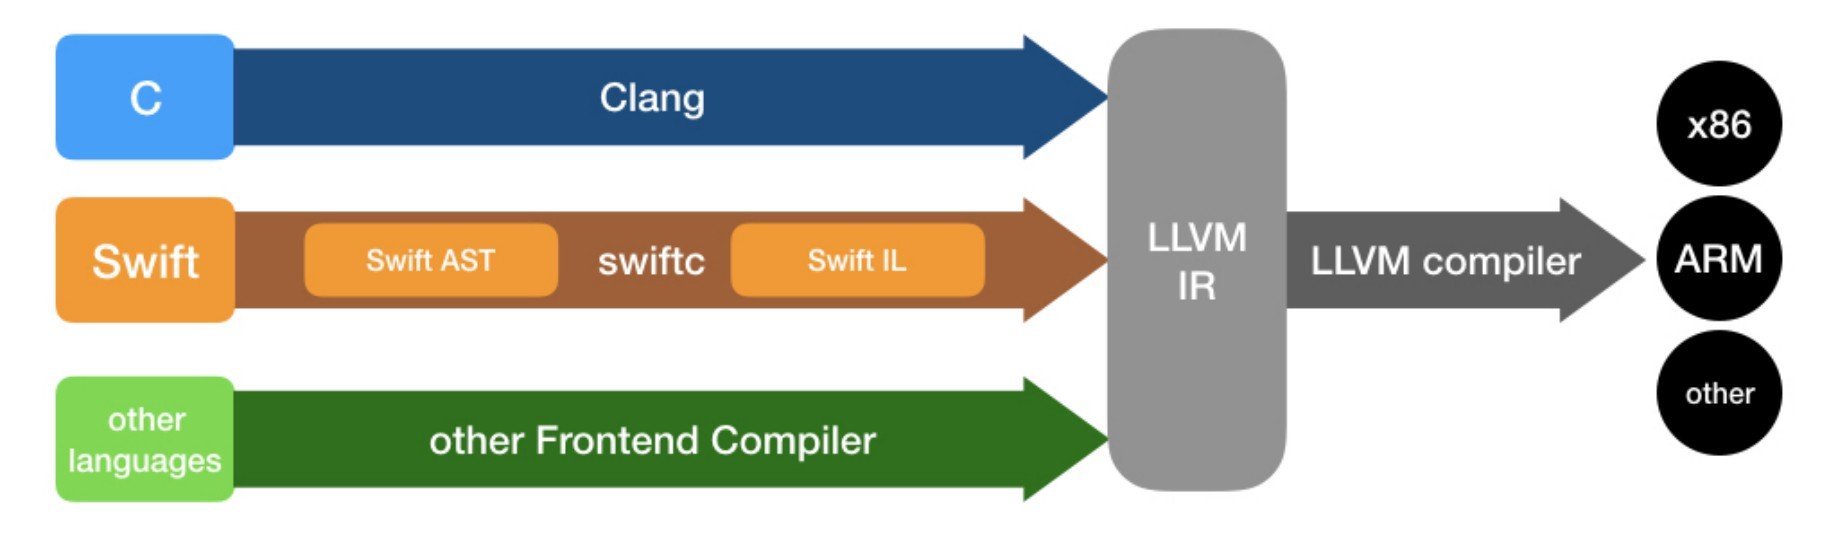
\includegraphics[height=\textheight, width=\textwidth, keepaspectratio=true]{beamerthemesrc/images/llvm-ir.png}
%         \caption{Exemplo de RI: LLVM-IR.}
%     \end{figure}
% \end{frame}

% \begin{frame}[fragile]{RI — Serde: Conversões automatizadas para JSON}
%     \begin{columns}
%         \begin{column}{.55\textwidth}
%             \begin{block}{Rust}
%                 \begin{lstlisting}[language=Rust]
% #[derive(Serialize, Deserialize)]
% struct Person {
%     name: String,
%     age: u8,
%     phones: Vec<String>,
%     address: Address,
% }
% #[derive(Serialize, Deserialize)]
% struct Address {
%     street: String,
%     city: String,
% }
%                 \end{lstlisting}
%             \end{block}
%         \end{column}

%         \begin{column}{.45\textwidth}
%             \begin{block}{JSON}
%                 \begin{lstlisting}[language=json, tabsize=2]
% {
%   "name": "John Doe",
%   "age": 43,
%   "address": {
%     "street": "1st St.",
%     "city": "London"
%   },
%   "phones": [
%     "+44 1234567",
%     "+44 2345678"
%   ]
% }
%                 \end{lstlisting}
%             \end{block}
%         \end{column}
%     \end{columns}
% \end{frame}

% \begin{frame}[fragile]{RI — \textit{Templates}}

%     \begin{itemize}
%         \item \texttt{Structs} \textit{serializáveis} podem ser usadas diretamente em \textit{templates};
%         \item Suponha a variável \texttt{people: Vec<Person>}:
%     \end{itemize}

%     \begin{block}{minijinja}
%         \begin{lstlisting}[language=jinja2]
% 
%     {{ person.name }}, {{ person.age }} anos.
%     Contato: 
%       {{ phone_nb }}
%       , 
%     
% 
%         \end{lstlisting}
%     \end{block}
% \end{frame}

